\subsection{Architecture}

The suggested architecture in figure \ref{fig:suggestedArchitecture} only supports a handful of MIPS instructions, and lacks support for jump instructions that was present in the previous exercise.
However, by adding a shifter to the ALU and a few additional muxes, mainly to the memory stage, the number of supported instruction can be radically improved from 9 to 29.

The resulting architecture, which includes a forwarding unit for highly improved performance can be seen in figure \ref{fig:cpuArchitecture} below.
The control signals are not drawn to keep the schematic readable, but they are passed through the pipeline registers as the other signals until they reach their destination stage.
Note that the jump and branch signals belong to the memory stage.

\begin{figure}[ht]
    \centering
    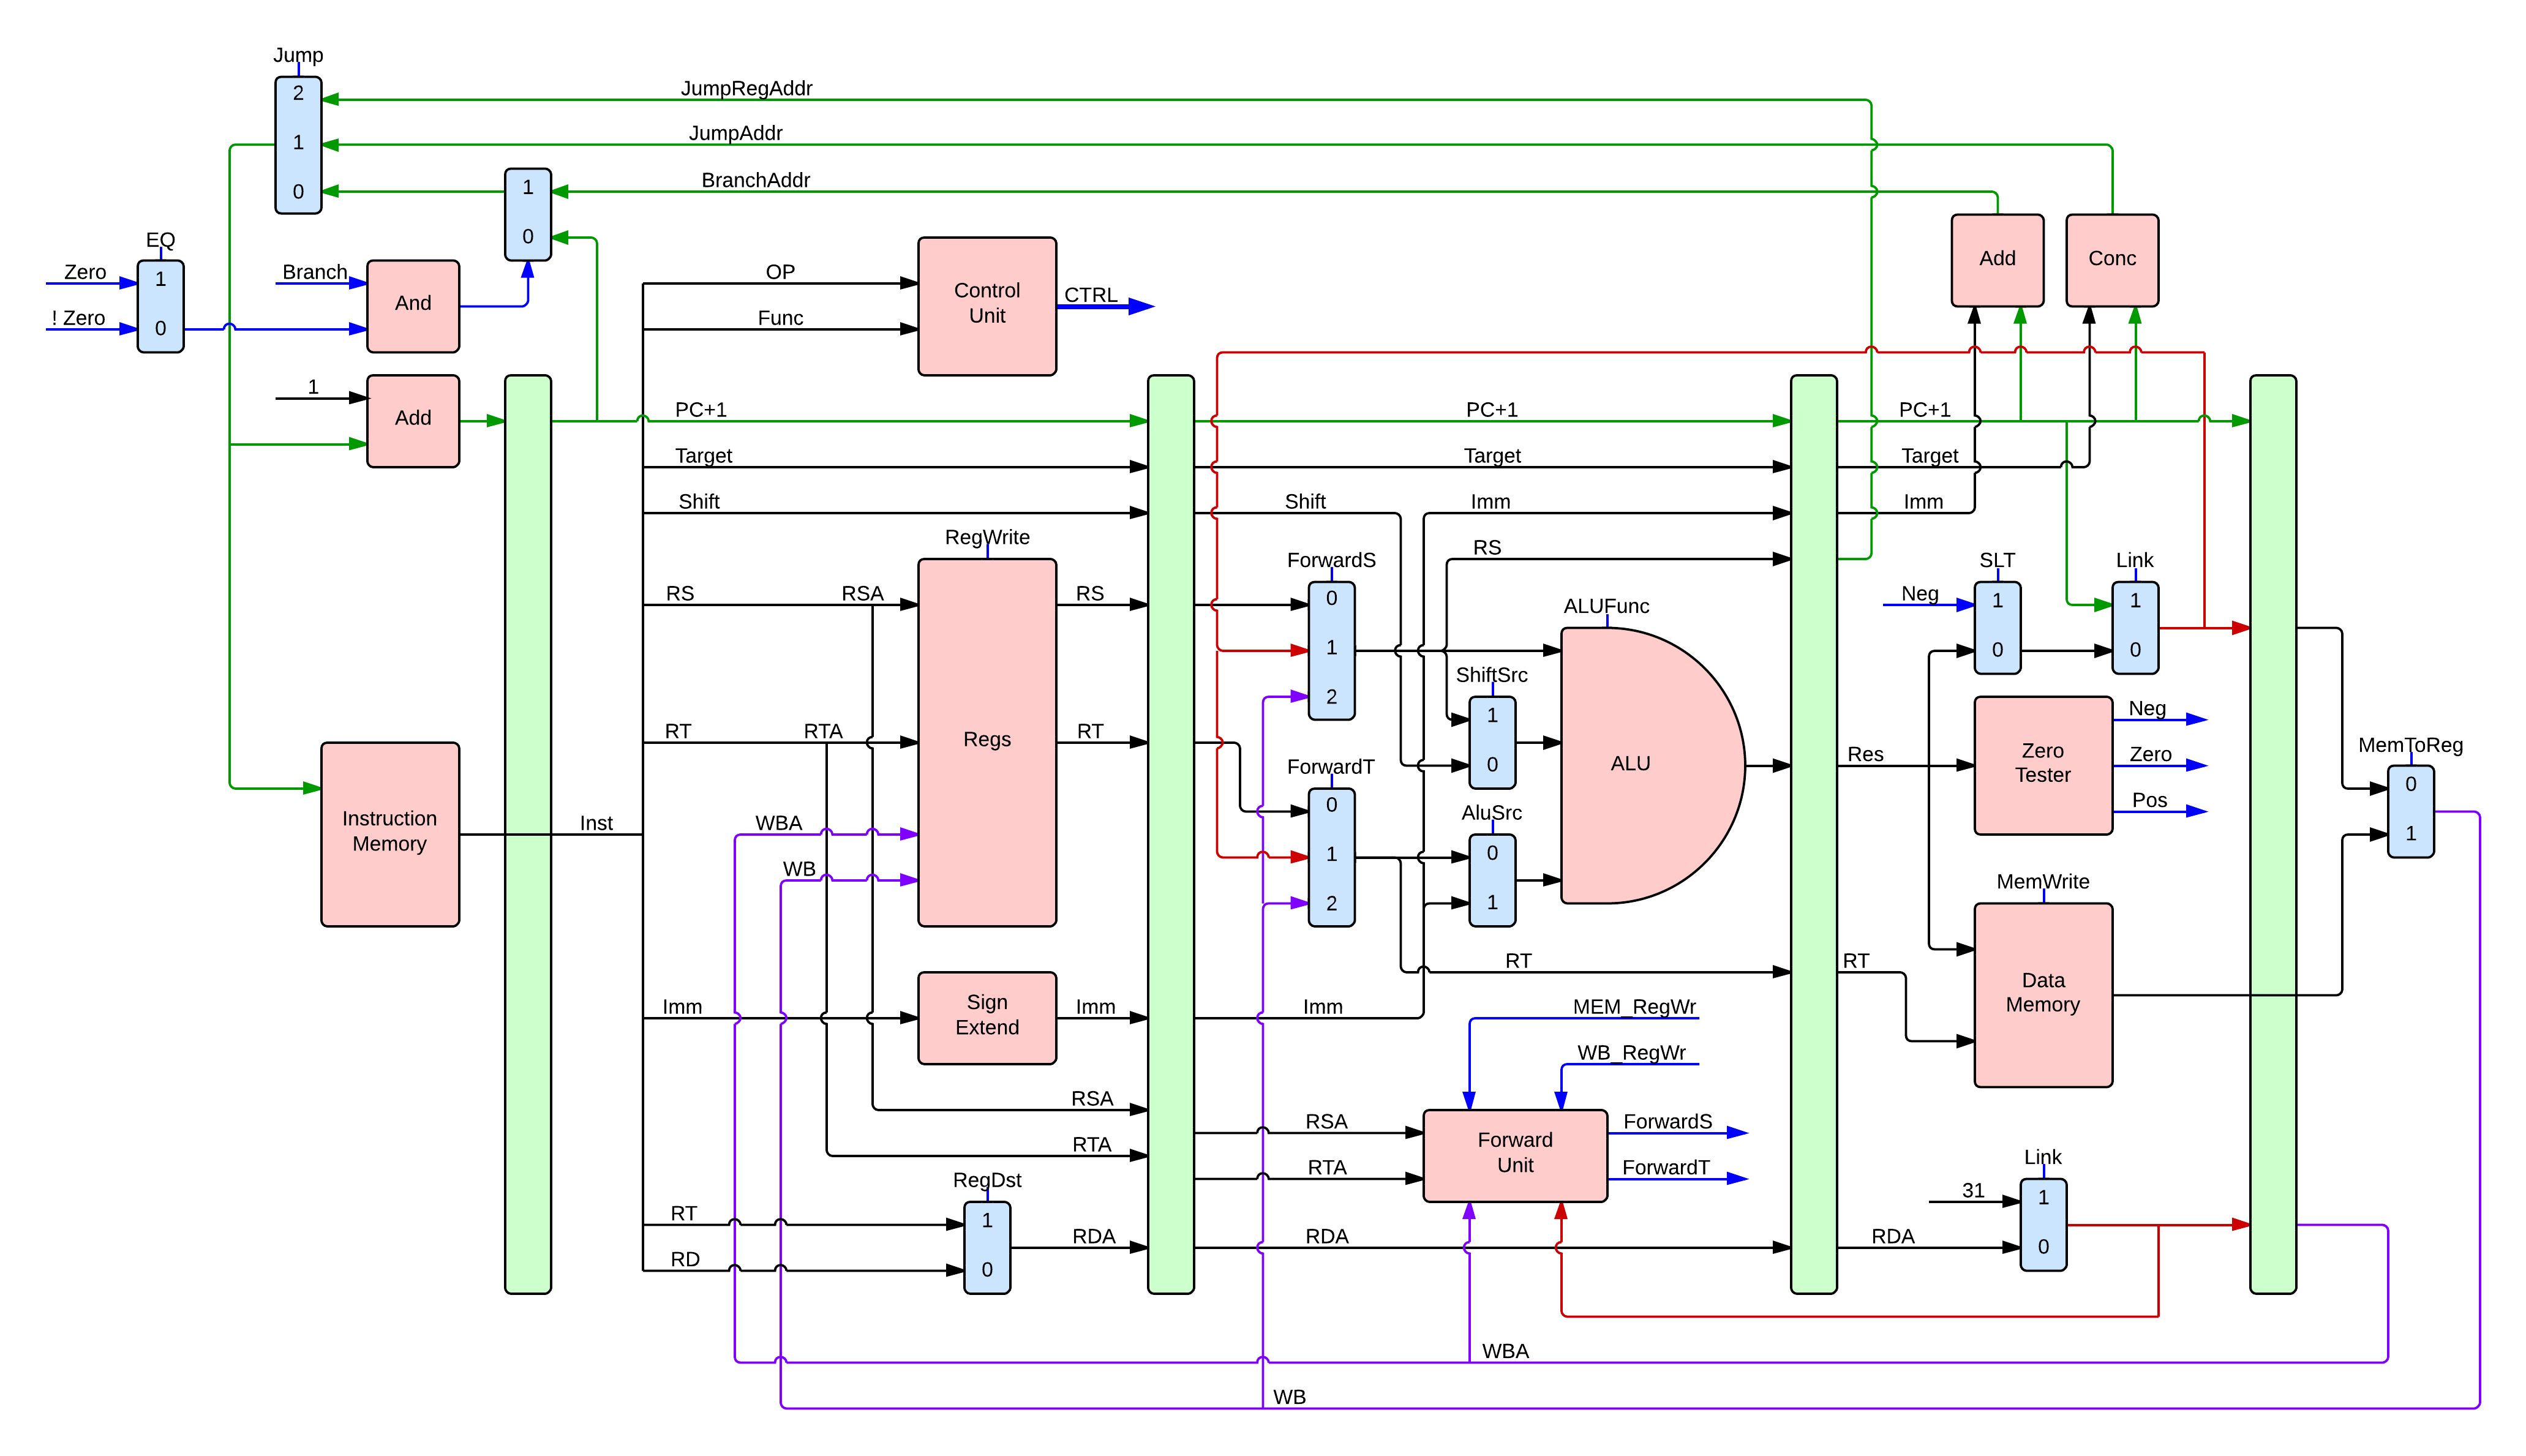
\includegraphics[width=\textwidth]{figures/Architecture.png}
    \caption{The implemented CPU architecture} 
    \label{fig:cpuArchitecture}
\end{figure}

There are a few things to note about this architecture.

First, since the instruction and data memories only read and write data on clock ticks, they act almost as pipeline registers for their own signals.
Therefore, their outputs are sent directly through the pipeline barrier to prevent the data from being delayed by an extra cycle.

Second, the address of the next instruction is fed directly into instruction memory to reduce latency, which allows the program counter to be merged into the first pipeline register.

Third, data from load word instructions is not forwarded from the memory stage and can therefore not be read in the following clock cycle.
This is a side effect of the data memory only acting on clock ticks.
Thus, to avoid reading invalid data, the instructions has to be reordered or a nop has to be added. This is normally accomplished by the assembler, which means it is hardly an issue.

\subsection{Instruction Set}

The instruction set is a reduced MIPS instruction set, supporting some
arithmetic and logics, both register bound and the immediate form, as well as
shifting, jumping, branching and load and store, totaling 29.

\subsubsection*{Control Unit}

Since the control signals are propagated to their proper stages through the pipeline, the control unit does not need a state machine like in multi-cycle processors.
It simply needs to look at the opcode and function to and then output the correct signals for that instruction.
All instructions and their control signal mappings can be seen below in table \ref{table:ctrlsignals}.
Note that there is no separate ALU control unit.

\begin{table}[ht]
    \begin{tabular}{|l|c|c|c|c|c|c|c|c|c|c|c|c|}
        \hline
        Instruction & B & EQ & J & L & SLT & RegDst & ShSrc & AluSrc & AluFun & MTR & RegW & MemW \\
        \hline
        add/addu   & 0 & X & 0 & 0 & 0 & 0 & X & 0 & Add & 0 & 1 & 0 \\
        sub        & 0 & X & 0 & 0 & 0 & 0 & X & 0 & Sub & 0 & 1 & 0 \\
        addi/addiu & 0 & X & 0 & 0 & 0 & 1 & X & 1 & Add & 0 & 1 & 0 \\
        \hline
        and        & 0 & X & 0 & 0 & 0 & 0 & X & 0 & And & 0 & 1 & 0 \\
        or         & 0 & X & 0 & 0 & 0 & 0 & X & 0 & Or  & 0 & 1 & 0 \\
        xor        & 0 & X & 0 & 0 & 0 & 0 & X & 0 & Xor & 0 & 1 & 0 \\
        nor        & 0 & X & 0 & 0 & 0 & 0 & X & 0 & Nor & 0 & 1 & 0 \\
        \hline
        sll        & 0 & X & 0 & 0 & 0 & 0 & 0 & 0 & SLL & 0 & 1 & 0 \\
        srl        & 0 & X & 0 & 0 & 0 & 0 & 0 & 0 & SRL & 0 & 1 & 0 \\
        sra        & 0 & X & 0 & 0 & 0 & 0 & 0 & 0 & SRA & 0 & 1 & 0 \\
        sllv       & 0 & X & 0 & 0 & 0 & 0 & 1 & 0 & SLL & 0 & 1 & 0 \\
        srlv       & 0 & X & 0 & 0 & 0 & 0 & 1 & 0 & SRL & 0 & 1 & 0 \\
        srav       & 0 & X & 0 & 0 & 0 & 0 & 1 & 0 & SRA & 0 & 1 & 0 \\
        \hline
        slt        & 0 & X & 0 & 0 & 1 & 0 & X & 0 & Sub & 0 & 1 & 0 \\
        slti       & 0 & X & 0 & 0 & 1 & 1 & X & 1 & Sub & 0 & 1 & 0 \\
        \hline
        j          & X & X & 1 & X & X & X & X & X & X   & X & 0 & 0 \\
        jal        & X & X & 1 & 1 & X & X & X & X & X   & X & 1 & 0 \\
        jr         & X & X & 2 & X & X & X & X & X & X   & X & 0 & 0 \\
        jral       & X & X & 2 & 1 & X & X & X & X & X   & X & 1 & 0 \\
        \hline
        beq        & 1 & 1 & 0 & X & X & X & X & 0 & Sub & X & 0 & 0 \\
        bne        & 1 & 0 & 0 & X & X & X & X & 0 & Sub & X & 0 & 0 \\
        \hline
        lui        & 0 & X & 0 & 0 & 0 & 1 & X & 1 & LUI & 0 & 1 & 0 \\
        lw         & 0 & X & 0 & 0 & 0 & 1 & X & 1 & Add & 1 & 1 & 0 \\
        sw         & 0 & X & 0 & 0 & X & X & X & 1 & Add & X & 0 & 1 \\
        \hline
    \end{tabular}
    \caption{Control signals for implemented instructions. Short notation due to space constraints: $ $ B = Branch, J = Jump, L = Link, MTR = MemToReg, RegW = RegWrite, MemW = MemWrite.}
    \label{table:ctrlsignals}
\end{table}


\subsection{Optimizations}
\subsubsection*{Forwarding Unit}
\todo{forwarding unit}

\subsubsection*{Branch Prediction}
\todo{branch prediction}

\subsection{Assembler}
An assembler was written in python to easily write more test programs. It
assumes the programmer knows what she is doing, and will not give nice error
messages. When given the flag '-x', the assembler writes the instructions on
hexadecimal form, to easily run the programs on the computer.
